\documentclass[tikz]{standalone}
\usepackage{tikz}
\usetikzlibrary{calc}

\usepackage{units}

\newcommand*{\Angle}{35}% 
\newcommand*{\Overshoot}{22.5}%
\newcommand*{\R}{2.5}%
\newcommand*{\LgthAx}{2.5}%
\newcommand*{\Lo}{-0.6}%
\newcommand*{\Sep}{0.18}%
\newcommand*{\YSep}{0.1}%
\newcommand*{\XSep}{0.2}%
\newcommand*{\DashLgth}{0.75}%

\begin{document}
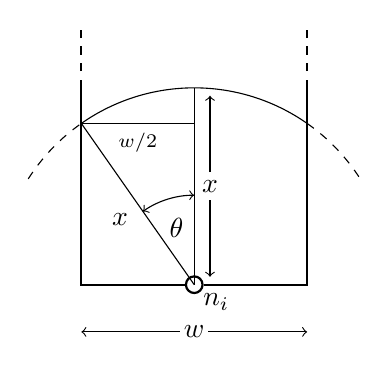
\begin{tikzpicture}


    % (theta:r) polar coordinates!

    \pgfmathsetmacro{\WdthAx}{\R*sin(\Angle)}%

    \node[draw, inner sep=0pt, minimum size = 6pt, circle, thick] at
    (0,0) (neuron) {};
    \draw[thick] (-\WdthAx,\LgthAx) -- (-\WdthAx,0) --
    (neuron) -- (\WdthAx,0) -- (\WdthAx,\LgthAx);

    \draw   (0,0) -- node[auto] {$x$} (90+\Angle:\R);
    \draw[dashed]  (90+\Angle+\Overshoot:\R) arc (90+\Angle+\Overshoot:90+\Angle:\R);
    \draw (90+\Angle:\R) arc (90+\Angle:90-\Angle:\R);
    \draw[dashed] (90-\Angle:\R) arc (90-\Angle:90-\Angle-\Overshoot:\R);

    \draw[<->] (90+\Angle:\R/2.2) arc (90+\Angle:90:\R/2.2); 
    \node at (90+\Angle/2:\R/2-0.5) {$\theta$};

    \draw[<-] (\WdthAx,\Lo) -- (0+\Sep,\Lo);
    \draw[<-] (-\WdthAx, \Lo) -- (0-\Sep,\Lo);
    \node at (0,\Lo) {$w$};

    \draw[<-] (\XSep,\YSep) -- (\XSep, \R/2-\Sep);
    \draw[->] (\XSep,\R/2+\Sep) -- (\XSep, \R - \YSep);
    \node at (\XSep,\R/2) {$x$};

    \node at (0.28,-0.22) {$n_i$};
    \draw (0,0) -- node[right]  {} (0,\R);

    \draw (90+\Angle:\R) -- node[below] {$\scriptstyle w/2$} ($(90+\Angle:\R)!.5!(90-\Angle:\R)$);

    \draw[thick, dashed] (-\WdthAx, \LgthAx) -- (-\WdthAx, \LgthAx + \DashLgth);
    \draw[thick, dashed] (\WdthAx, \LgthAx) -- (\WdthAx, \LgthAx + \DashLgth);


\end{tikzpicture}
\end{document}
%%% Local Variables: 
%%% mode: latex
%%% TeX-master: t
%%% End: 
